\section{Problem B}
\textit{The achievable transmission rate R (bits/s) in a channel of bandwidth W (Hz) is related to the transmission power P (W) and noise power spectral density No (W/Hz) through the Shannon-Hartley formula:}
\begin{flalign}
 && R=& W\,\log_2\left(1+\frac{P}{W\,N_0}\right) &
\end{flalign}

\subsection{1)}
\textit{From the quantities entering the Shannon-Hartley formula, define Spectral Efficiency (SE), $\eta_{SE}$, in bps/Hz. Next, derive the trade-off between spectral efficiency and transmitted energy per bit, $E_b$. Plot the relation between SE and energy per bit, and conclude what is the best strategy in terms of minimising the energy consumption for a given fixed transmission rate R. As part of this, what is the minimum possible energy consumption per bit?}\\

By definition the Spectral Efficiency (SE) is given by the ratio between the bit Rate (R) and the Bandwidth. Using the Shannon formula the SE is:
\begin{flalign}
 && \eta _{SE}=& \frac{R}{W}= \,\log_2\left(1+\frac{P}{W\,N_0}\right) &
\end{flalign}
In order to get the trade-off between spectral efficiency and transmitted energy per bit the following steps are executed.\\
The energy per bit is given by:
\begin{flalign}
 && E_b=& \frac{P}{R} &
\end{flalign}
The Power is exact from the equation 12.4:
\begin{flalign}
 && 2^{\eta _{SE}}=& \left(1+\frac{P}{W \cdot N_0}\right) &\\
 && P=& \left(2^{\eta _{SE}}-1\right)W\cdot N_0 & 
\end{flalign}
So, the equation 12.5 became as:
\begin{flalign}
&& E_b=& \dfrac{\left(2^{\eta _{SE}}-1\right)W\cdot N_0}{R} & \\
 &&=& \dfrac{\left(2^{\eta _{SE}}-1\right)\cdot N_0}{\eta _{SE}}
\end{flalign}
In the figure 12.1 is plotted the relation between SE and energy per bit.
\begin{figure}[!h]
  \centering
  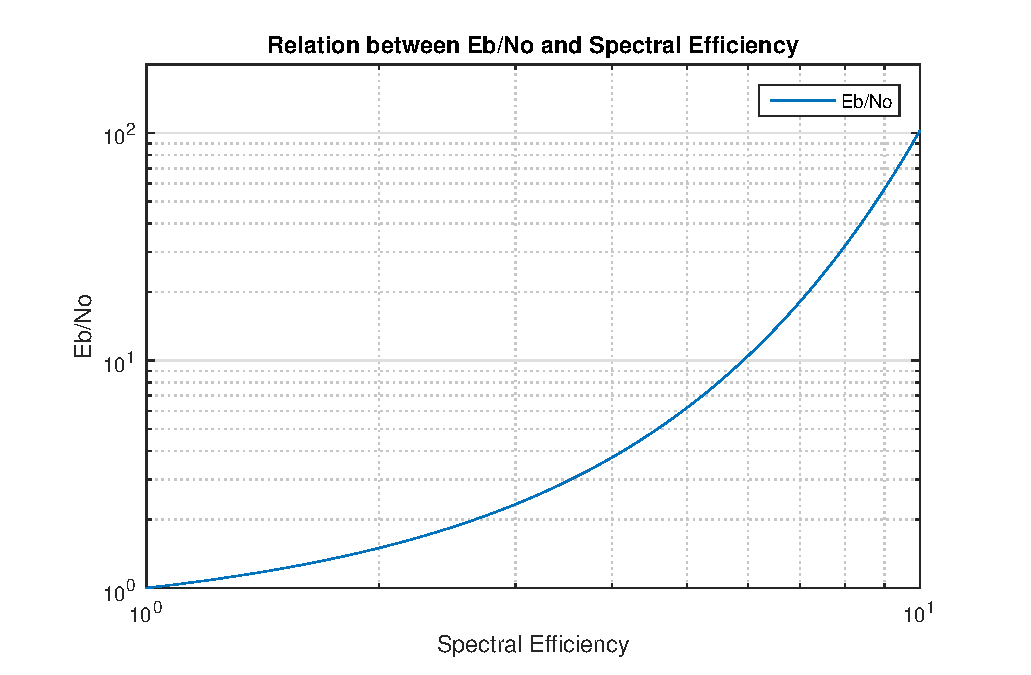
\includegraphics[width=14cm]{mm12-1b1.eps}
  \caption{Relation between SE and energy per bit}
  \label{fig:SE_Eb}
\end{figure}
In order to minimize the energy consumption with a fixed Bit Rate is necessary have a small spectral efficiently, which means have a wide bandwidth.
\newpage
\subsection{2)}
\textit{Derive the trade-off between Spectral Efficiency (SE) and Energy Efficiency (EE) based on the Shannon-Hartley formula: Define EE, $\eta_{EE}$, in bits/Joule (naturally you would perhaps define Joule/bit, which however complicates things a bit), and then relate them via the formula.}\\

SOMETHING...\\

\textit{Sketch the relation in a graph and conclude whether it is possible to simultaneously maximise both quantities. As part of this, what happens to EE when SE approaches $0$ and $\infty$ (infinity), respectively?}\\

VERY NICE SKETCH...\\

\textit{The relation is a purely theoretical one which neglects several practical limitations, such as…?}\\

SOMETHING...


